On the whole, the implementation can be divided into two parts: client and server. Since they are fully separated, each part is considered and structured as a independent project. The implementation on client side is basically data fetching and template rendering, while data persistence and core business logic is implemented on the server side.  For convenience, the graphical discuss system is named \textbf{"Graphicuss"}, which stands for graphical plus discuss.


\subsection{Platform and Framework}
To achieve a better performance of view rendering on client side running in browser, ReactJS\footnote{https://facebook.github.io/react/} is taken as the front-end framework. Componentization, the main philosophy of ReactJS, also helps organize the views and view model logics. On the server side, ExpressJS\footnote{http://expressjs.com/} as a web framework is adopted for its efficiency and productivity of building RESTFul APIs.

Since both client and server projects are primarily implemented in JavaScript, NodeJS\footnote{https://nodejs.org/} is the single development environment for either project implementation or project management on both sides.

\subsubsection{File Structure}

To have a basic understanding of whole project including the server side and client side, a file structure of the project Graphicuss is listed in figure \ref{fig:overview-file-structure}:

\begin{itemize}
\item 
  \textbf{client/}: independent front-end project built on top of ReactJS
\item
  \textbf{server/}: independent back-end project implemented by using ExpressJS
\item
  \textbf{dist/}: compiled back-end project integrated with compiled and compressed static view files from front-end project
\item 
  \textbf{node\_modules/}: source of referenced third party libraries
\item 
  \textbf{package.json}: definition of third party libraries for client and server side
\item 
  \textbf{webpack.config.json}: config of specific behaviours in automated development or building process
\end{itemize}

\begin{figure}[!htbp]
\centering
\begin{forest}
  for tree={
    font=\ttfamily,
    grow'=0,
    child anchor=west,
    parent anchor=south,
    anchor=west,
    calign=first,
    edge path={
      \noexpand\path [draw, \forestoption{edge}]
      (!u.south west) +(7.5pt,0) |- node[fill,inner sep=1.25pt] {} (.child anchor)\forestoption{edge label};
    },
    before typesetting nodes={
      if n=1
        {insert before={[,phantom]}}
        {}
    },
    fit=band,
    before computing xy={l=15pt},
  }
[Graphicuss
  [client/]
  [server/]
  [dist/]
  [node\_modules/]
  [package.json]
  [webpack.config.js]
]
\end{forest}
\caption{Overview of Graphicuss' file structure}
\label{fig:overview-file-structure}
\end{figure}


\subsubsection{Module Management}

NodeJS provides native module management which is called \textit{npm}\footnote{https://www.npmjs.com}. Third party libraries, which are published in the official remote repository, can be installed conveniently by only using npm's command line. There is also a list of names of all modules and dependencies in the file \textit{package.json}. Installing all dependencies and modules can be simply achieved by using only one command line \textit{npm install}, which will significantly ease the setting up process of the project freshly on a new machine.

\subsection{Architecture}

An architectural overview of Graphicuss is illustrated in figure \ref{fig:general-arch-imp}.

\begin{figure}[!htbp]
  \centering
    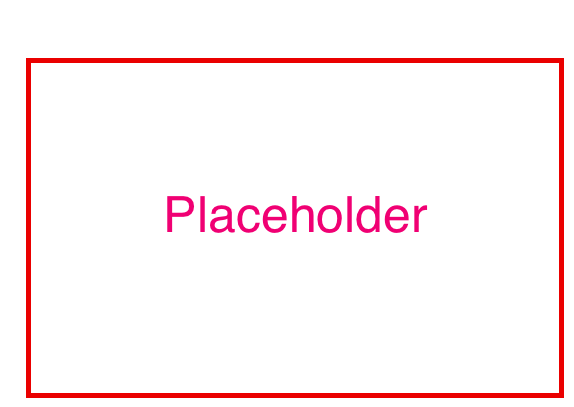
\includegraphics[width=0.6\textwidth]{Figures/placeholder.png}
  \caption{placeholder}
  \label{fig:general-arch-imp}
\end{figure}
% Big Pic! Client with xuxian circle domain + React Engine -> Router in Express -> logic business + Database -> return 
While the client starts requesting a specific URL for data from the server, a HTTP connection will be established. The server program receives the HTTP request and forwards it to its router, in which rules for matching URLs have been pre-defined. By analysing headers of HTTP request, router will check if the request matches any pre-defined rules.

Not only the URL but also the parameters passed by client, for example the identifier of a resource, could also be extracted from HTTP headers. Server runs correlate business logics according to the rule of matched URL and executes operations of databases for data persistence. Afterwards, results are returned from server.

As soon as the data is successfully returned, the HTTP connection will be closed. The client processes data acquired from server, and represents it by re-rendering views. So far, a entire request over HTTP is accomplished.

\subsection{Automatization}
To accelerate the developing as well as building process of the project, a automatization tool called \textit{Webpack}\footnote{https://webpack.github.io/} is used. 

Webpack is a tool which could analyse the dependencies of the project and bundle modules with the app. In addition, it can also do tasks like compressing JavaScript codes to reduce the size of the client app, or compiling modern JavaScript as well as CSS codes to achieve the compatibility for old browsers.

\subsubsection{Automated Development Process}
To make the development of client app independent, it will start a dev server on its own for development purpose. However the dev server started by client app and the actual server are running on different ports. Which means that the communication between them will cause CORS problem.

CORS means, a resource makes a cross-origin HTTP request when it requests a resource from a different domain than the one which the first resource itself serves. For security reasons, browsers restrict cross-origin HTTP requests initiated from within scripts. \cite{CORS}

Through configuring the dev server started by Webpack, a proxy could established to forward request to the actual back-end server. As figure \ref{fig:proxy-server-imp} shows, the client is able now to request APIs under the same domain, and requests will go though the dev server, after that they are forwarded to the actual server.

\begin{figure}[!htbp]
  \centering
    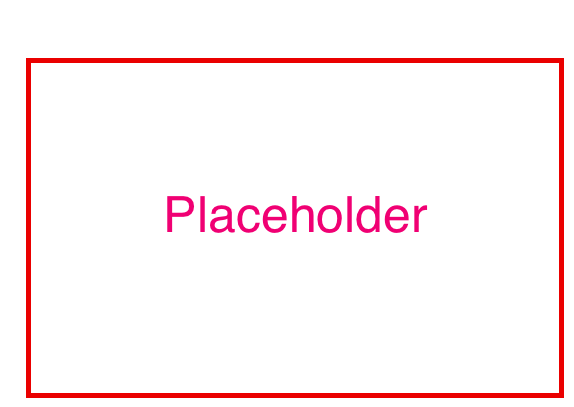
\includegraphics[width=0.6\textwidth]{Figures/placeholder.png}
  \caption{placeholder}
  \label{fig:proxy-server-imp}
\end{figure}
% Dev Process, in development(dev server, proxy) + building)


\subsubsection{Automated Building Process}

For the client app, multiple tasks are executed during the building process by using Webpack: transforming modern JavaScript code, pre-processing the modern CSS code and bundling the static files. All these tasks will significantly reduce the size of client app and also improve the compatibility of the app.

The usage of Webpack on server app is quite different. It will bundle all dependencies with the server app. After processing on both sides, the final output of the files will be extracted into the \textit{dist} directory mentioned in \ref{fig:overview-file-structure}, which is now ready for deploying and serving. The whole building process is represented in figure \ref{fig:automated-building-imp}.

\begin{figure}[!htbp]
  \centering
    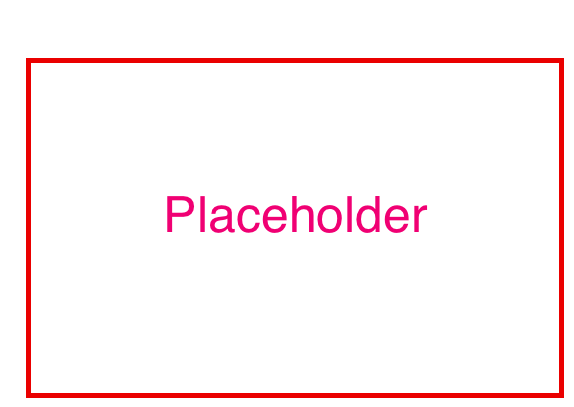
\includegraphics[width=0.6\textwidth]{Figures/placeholder.png}
  \caption{placeholder}
  \label{fig:automated-building-imp}
\end{figure}
% Building Process, a->b->c->d xuxian kuang, Webpack compile, bundle, compress -> copy file to dist -> ready for deploy

\subsection{Storage Structure} \label{subsec:storage-structure-imp}
In section \ref{sec:data-concept}, data domains and fields of data domains  have already been defined. 

For all persistence storage of data on the server side a MongoDB\footnote{https://www.mongodb.com/} database is used.  In figure \ref{fig:data-model-table-imp}, more concrete definition of data model table is defined. MongoDB is a non-SQL database, which uses document oriented storage and JSON style data model. That will make it easy to implement as well as scale data models. In addition, An \gls{ORM} framework called Mongoose\footnote{http://mongoosejs.com/} is also applied to the implementation, which encapsulates the native database operations of MongoDB. With help of the \gls{ORM} framework, definition of schema and query on database will be quite simple. 

% Description othe the table?

\begin{figure}[!htbp]
  \centering
    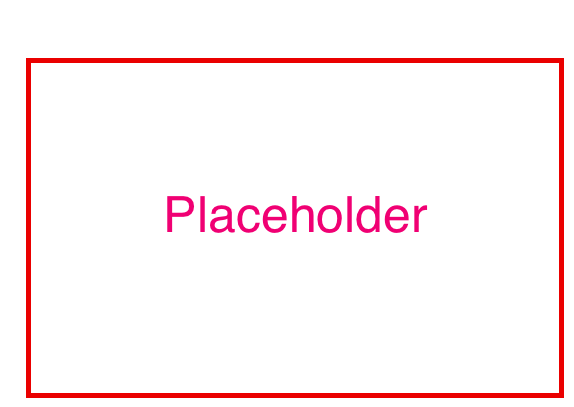
\includegraphics[width=0.6\textwidth]{Figures/placeholder.png}
  \caption{placeholder}
  \label{fig:data-model-table-imp}
\end{figure}
% Whole Concret Data Model Table
